\chapter{Analyse et recommandations}
\label{chap:4}
\sloppy

\section{Analyse des cas de succès et d'échec}

Dans l'ensemble, il a été observé qu'une classe, à savoir AFV, a bien fonctionné dans nos deux expériences.
La raison en est que cette classe avait plus de données d'entraînement que les autres classes.
Les détails de notre ensemble de données proposé sont donnés dans le tableau \ref{tab:label_data}.
Au cours de l'analyse, nous avons observé que le système avait de bonnes performances sur les cas de test sur les images avec des véhicules visibles, mais il y avait des difficultés dans certains cas pour lesquels nous avions un petit jeu de données d'entraînement.
Il fonctionne bien sur les véhicules militaires dans les données non vues par rapport aux autres véhicules militaires car le rapport entre ses données d'entraînement est plus élevé.

Le modèle commence à mal fonctionner sur des données. Cela est dû au fait qu'il y a moins de données d'entraînement par rapport à l'autre classe.

\begin{table}[H]
    \centering
    \begin{tabular}{|l|l|l|p{2.8cm}|p{2cm}|p{2cm}|p{2cm}|}
        \hline
        \textbf{Label} & \textbf{Quantité} & \textbf{Pourcentage} & \textbf{Modèles} & \textbf{Précision moyenne} & \textbf{Recall moyen} & \textbf{F1-Score moyen} \\ \hline
        AFV            & 6694              & 82.5\%               & YoloV8 (m et l)  & 0.71                       & 0.676                 & 0.69                    \\ \hline
        APC            & 1212              & 15.0\%               & YoloV8 (m et l)  & 0.58                       & 0.544                 & 0.557                   \\ \hline
        LAV            & 374               & 4.6\%                & YoloV8 (m et l)  & 0.52                       & 0.464                 & 0.49                    \\ \hline
        MEV            & 123               & 1.5\%                & YoloV8 (m et l)  & 0.29                       & 0.530                 & 0.374                   \\ \hline
    \end{tabular}
    \caption{Tableau des moyennes des résultats}
    \label{tab:label_data}
\end{table}


\section{Limites et perspectives}
\subsection{Modèle de détection d'objets}

Ici, le modèle YoloVx, grâce à plusieurs contributions, a connu un gain de performance considérable durant ces dernières années.
Nous avons des scores de précision d'environ 80\% malgré la faible quantité de données utilisée pour l'entraînement du modèle.
Néanmoins, les paramètres (hyperparamètres) de ces modèles deviennent plus complexe à comprendre et à personnaliser et à améliorer afin d'obtenir des résultats optimales adapter à nos besoins.
A ce jour, par rapport à nos contraintes en détection de véhicules militaires, YoloVx c'est le modèle de détection me plus performant.
Nous allons continuer à ajuster les paramètres pour obtenir un modèles beaucoup plus performant.

\subsection{Augmentation des données}
\subsubsection{Transformation des images}
\label{trando_image}
Dans cette étapes, nous appliquons trois transformations (scale, XYMasking, et Météo).
Grâce à cette méthode, en l'appliquant sur toutes les images du jeu de données, nous avons presque doublé leur nombre ainsi que leur annotation pour l'entraînement de notre modèles.

Nous avons fait un contrôle de qualité des images,nous avons constaté qu'il ya des images impossibles à lire.
Le tri de ces images n'est pas envisageable au vue de la quantité (3335) d'images du jeu de données sur le quel les transformations ont été appliquées.


\begin{figure}[H]
    \centering
    \begin{subfigure}[b]{0.4\textwidth}
        \centering
        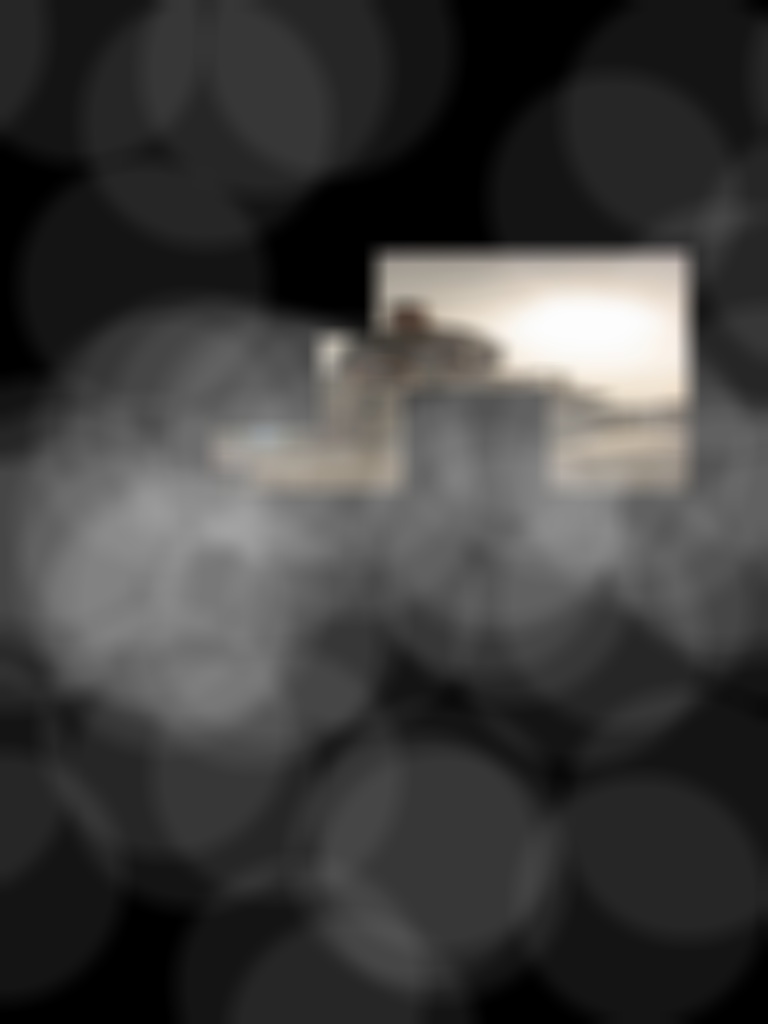
\includegraphics[height=4cm]{./images/augmented-1.jpg}
    \end{subfigure}
    \hfill
    \begin{subfigure}[b]{0.4\textwidth}
        \centering
        
\includegraphics[height=4cm]{./images/augmented-2.jpg}
    \end{subfigure}
    \vskip\baselineskip
    \begin{subfigure}[b]{0.4\textwidth}
        \centering
        
\includegraphics[height=4cm]{./images/augmented-3.jpg}
    \end{subfigure}
    \hfill
    \begin{subfigure}[b]{0.4\textwidth}
        \centering
        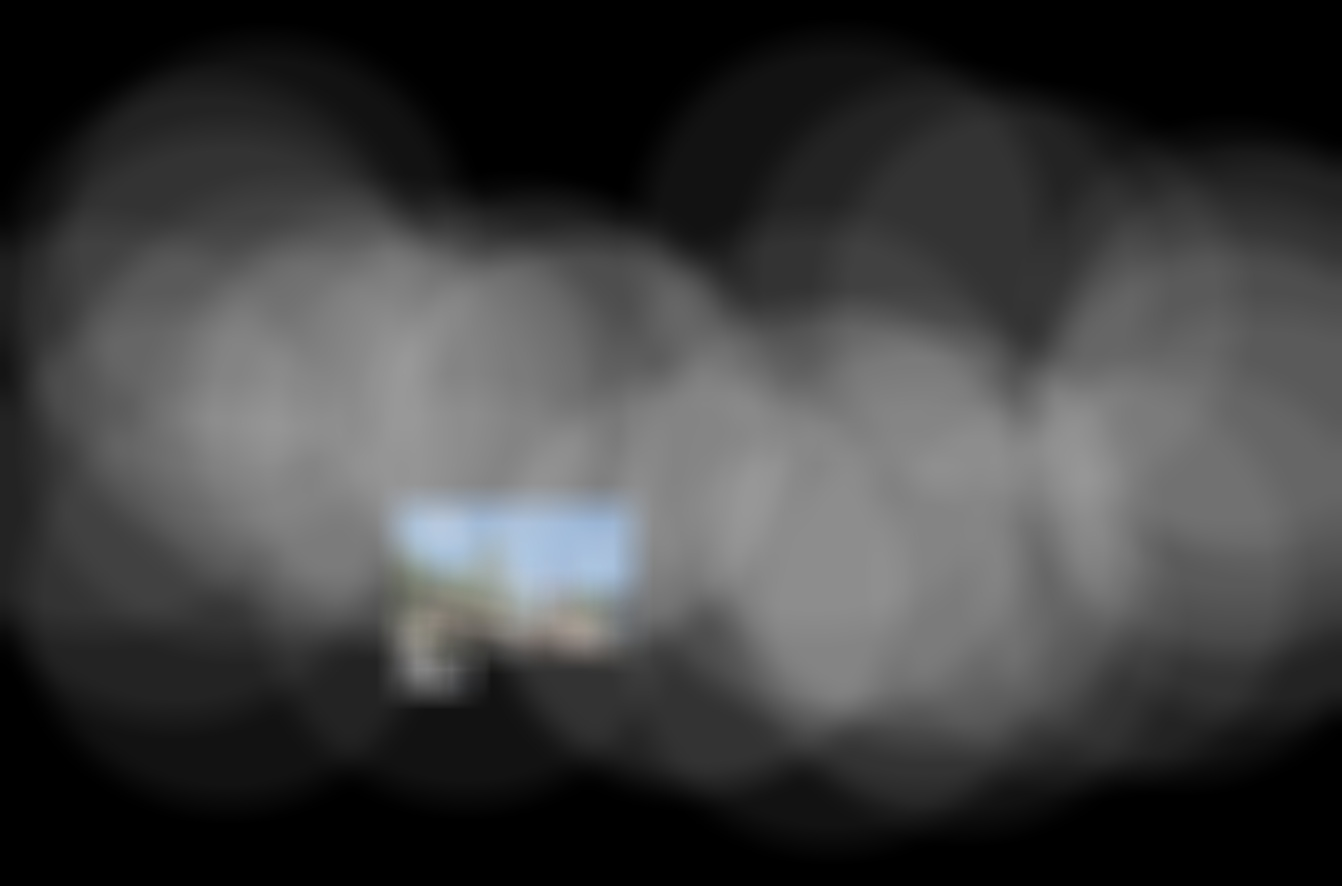
\includegraphics[height=4cm]{./images/augmented-4.JPEG}
    \end{subfigure}
    \caption{Exemples d'images transformées de véhicules militaires inexploitables}
    \label{fig:image_floues}
\end{figure}


\subsubsection{Génération d'images}

La génération d'image nous permet d'augmenter le nombre de véhicules de notre jeu de données.
Comme inconvénients, sous pouvons citer :

\begin{itemize}
    \item Elle ne peut générer qu'un seul type de véhicule.
    \item Beaucoup d'images ne sont pas réalistes par conséquent inexploitables.
    \item Les images ne sont pas annotées et nécessite une annotation manuelle.
    \item Aucun moyen d'évaluer objectivement la qualité du rendu. Tout est subjectif, donc fastidieux.
\end{itemize}

\begin{quote}
    % \textit{Si vous recherchez un certain résultat dans votre art, déterminer si un modèle est sur ou sous-entraîné sera toujours subjectif, car l'art est subjectif.}\\
    \textit{If you are going for a certain result in your art, then determining if a model is over or under trained is always going to be subjective, because art is subjective.\cite{reddit_proverbe}}
\end{quote}


\begin{figure}[H]
    \centering
    \begin{subfigure}[b]{0.45\textwidth}
        \centering
        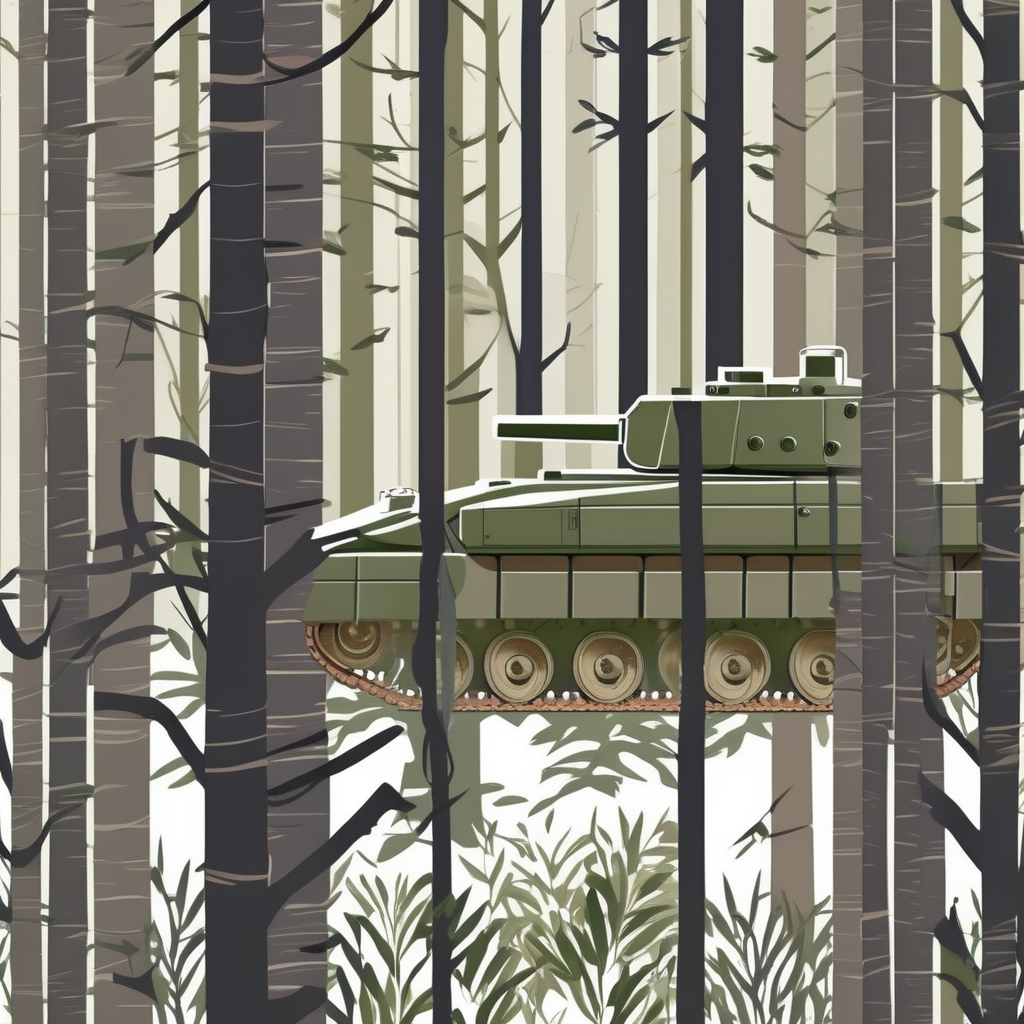
\includegraphics[height=5cm]{./images/tank-forest_camouflage-1.png}
    \end{subfigure}
    \hfill
    \begin{subfigure}[b]{0.45\textwidth}
        \centering
        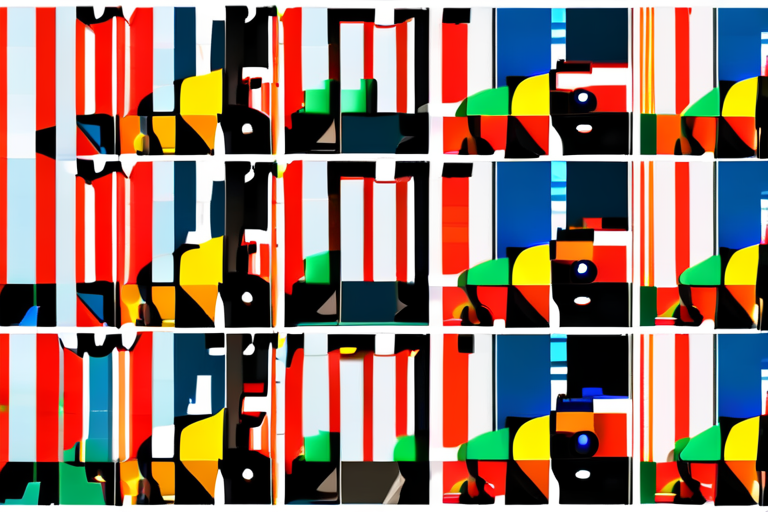
\includegraphics[height=5cm]{./images/tank-night_operation-1.png}
    \end{subfigure}
    \vskip\baselineskip
    \begin{subfigure}[b]{0.45\textwidth}
        \centering
        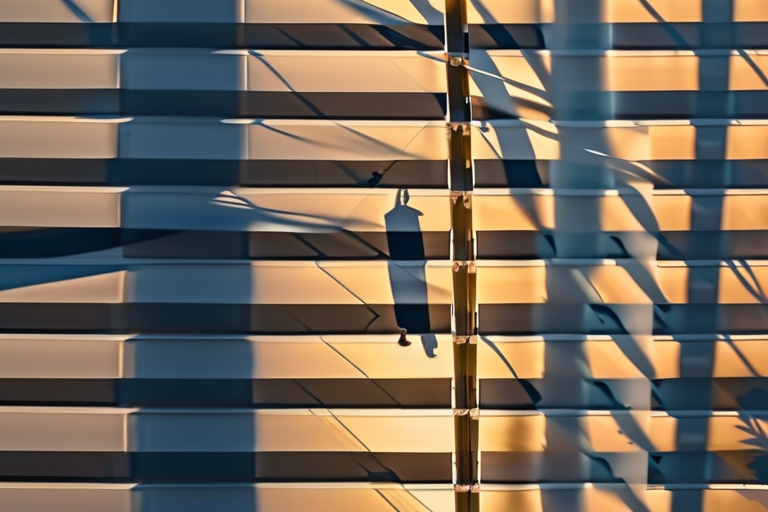
\includegraphics[height=5cm]{./images/tank-sunrise_maneuver-1.png}
    \end{subfigure}
    \hfill
    \begin{subfigure}[b]{0.45\textwidth}
        \centering
        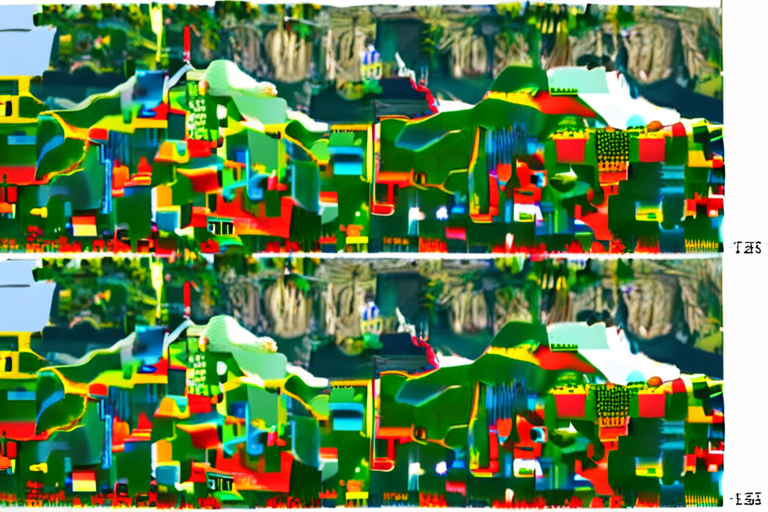
\includegraphics[height=5cm]{./images/tank-mountain_path-0.png}
    \end{subfigure}
    \caption{Exemples d'images synthétiques de véhicules militaires irréalistes et inexploitables}
\end{figure}


\subsection{Evolution des résultats}

Il est important de noter une dégradation significative des performances lors de l’utilisation des techniques de data augmentation, comme observé dans la section \ref{results-prepare03}.
En effet, alors que l’on aurait pu s’attendre à une amélioration des résultats avec l’ajout d’images augmentées, les performances du modèle se sont dégradées.
On passe ainsi d’un mAP de 0.66 sans data augmentation, avec des f1-scores respectables pour les différentes classes AFV: 0.8, APC: 0.7, LAV: 0.62, MEV: 0.67 (\textbf{Tableau \ref{tab:map-train-01}}), à un mAP de 0.34 avec data augmentation, et des f1-scores réduits AFV: 0.68, APC: 0.58, LAV: 0.46, MEV: 0.29 (\textbf{Tableau \ref{tab:results_moy_prepare03}}). \\

\newcolumntype{C}[1]{>{\centering\arraybackslash}p{#1}}

\begin{table}[H]
    \centering
    \begin{tabular}{|C{1.5cm}|C{1.8cm}|C{1.5cm}|C{2cm}|C{1.8cm}|C{1.5cm}|C{2cm}|}
        \hline
        \multirow{2}{*}{\textbf{Classes}} & \multicolumn{3}{c|}{\textbf{Sans data augmentation}} & \multicolumn{3}{c|}{\textbf{Avec data augmentation}}                                                                                             \\ \cline{2-7}
                                          & \textbf{Précision}                                   & \textbf{Recall}                                      & \textbf{F1-score} & \textbf{Précision}    & \textbf{Recall}       & \textbf{F1-score}     \\ \hline
        AFV                               & \textbf{0.76}                                        & \textbf{0.85}                                        & \textbf{0.80}     & \textcolor{red}{0.71} & \textcolor{red}{0.66} & \textcolor{red}{0.68} \\ \hline
        APC                               & \textbf{0.69}                                        & \textbf{0.72}                                        & \textbf{0.70}     & \textcolor{red}{0.59} & \textcolor{red}{0.57} & \textcolor{red}{0.58} \\ \hline
        LAV                               & \textbf{0.55}                                        & \textbf{0.72}                                        & \textbf{0.62}     & \textcolor{red}{0.51} & \textcolor{red}{0.41} & \textcolor{red}{0.46} \\ \hline
        MEV                               & \textbf{0.62}                                        & \textbf{0.71}                                        & \textbf{0.67}     & \textcolor{red}{0.22} & \textcolor{red}{0.40} & \textcolor{red}{0.29} \\ \hline
        \textbf{mAP}                      & \multicolumn{3}{c|}{\textbf{0.6609}}                 & \multicolumn{3}{c|}{\textcolor{red}{0.3425}}                                                                                                     \\ \hline
    \end{tabular}
    \caption{Comparaison des résultats sans et avec data augmentation}
    \label{tab:comparaison_aug}
\end{table}


L'analyse des images augmentées a révélé qu’un grand nombre d’entre elles étaient floues (Ex. Figures \ref{fig:image_floues}), comme cela a été observé dans la section \ref{trando_image}.
Cette dégradation de qualité pourrait provenir des paramètres de transformations, telles que l’ajout de brouillard ou de distorsions, qui, bien que censées simuler des conditions environnementales variées, ont pu altérer la qualité des images.
Il est probable que ces images floues aient perturbé le modèle, réduisant ainsi sa capacité à reconnaître correctement les objets, en particulier les classes avec peu de d'images comme MEV et LAV, où la performance a chuté.\\

\noindent Quelques solutions envisageables :

\begin{itemize}
    \item Revoir les paramètres des transformations appliquées, notamment en réduisant l’intensité ou la fréquence d’apparition des effets de brouillard.
    \item Retirer certaines transformations spécifiques (comme le brouillard) afin de tester si elles ont un impact négatif sur les performances.
    \item Générer des images augmentées avec des transformations moins agressives tout en conservant la diversité des conditions environnementales.
    \item Enfin, trier manuellement les images augmentées pour écarter celles qui sont inutilisables
\end{itemize}



\section{Recommandations}
Nous avons proposer quelques pistes d'amélioration pour ce projet

\begin{itemize}
    \item \textbf{Transformation d'image:} Nous avons recommander dans un premiers temps de limité les transformations à 02 types par images au lieu de 03. Avec cela nous réduisons la probabilité d'obtenir des images complètement floues et inexploitable. En plus, cela peut nous permettre de faire de fois d'images en faisant des combinaisons de 02 types de transformations, nous aurons à la fin de la transformation 03 fois plus d'images dans le jeu de données.
    \item \textbf{Images synthétiques:} Stable diffusion V3 et XL, semblent générer des images moins réalistes de la version 1.5. On pourra se concentrer dans un premier temps sur cette version avant de passer aux versions plus récentes.
    \item \textbf{Jeux vidéos:} explorer la possibilité d'extraire des images de véhicules militaires dans des jeux vidéos.
    \item \textbf{Films d'actions/guerres: } En plus d'avoir des images réalistes, nous pourrons aussi avoir plusieurs images en situation complexe (camouflage, explosion, ...). Développer un outils permettant de couper des séquences vidéos contenant des scènes de guerres afin d'extraire le maximum d'images.
    \item \textbf{Vidéos des réseaux sociaux: } Scruter des publication pouvant contenir les images et ou vidéos contenant des véhicules militaires en situation complexe à reproduire.
\end{itemize}

Nous tenons à rester objectifs dans nos recommandations car, les images issues de ce travail, en majorité, ne seront pas annotées  et demandera donc un travail supplémentaire d’annotation manuelle, qui est souvent très coûteux (à minima en temps).















































\chapter{Analyse et recommandations}
\label{chap:4}
\sloppy

\section{Analyse des cas de succès et d'échec}

Dans l'ensemble, il a été observé que la classe \textbf{AFV} a bien fonctionné dans nos deux expériences. Cela s'explique par une plus grande quantité de données d'entraînement disponibles pour cette classe, comparée aux autres classes. Les détails de notre ensemble de données sont présentés dans le tableau \ref{tab:label_data}. 

Lors de l'analyse, nous avons noté que le modèle présentait de bonnes performances dans les cas où les véhicules étaient bien visibles. Toutefois, des difficultés sont apparues dans des situations où le jeu de données d'entraînement était limité, notamment pour les classes \textbf{MEV} et \textbf{LAV}. Le modèle s'est avéré particulièrement performant sur les véhicules militaires pour lesquels un plus grand nombre de données d'entraînement avait été fourni, par opposition aux autres types de véhicules.

Cependant, le modèle a montré des signes de faiblesse dans certaines conditions. Cela peut être directement lié au déséquilibre des données d'entraînement, avec une proportion significativement plus faible d'exemples pour les classes \textbf{MEV} et \textbf{LAV}.

\begin{table}[H]
    \centering
    \begin{tabular}{|l|l|l|p{2.8cm}|p{2cm}|p{2cm}|p{2cm}|}
        \hline
        \textbf{Label} & \textbf{Quantité} & \textbf{Pourcentage} & \textbf{Modèles} & \textbf{Précision moyenne} & \textbf{Recall moyen} & \textbf{F1-Score moyen} \\ \hline
        AFV            & 6694              & 82.5\%               & YoloV8 (m et l)  & 0.71                       & 0.676                 & 0.69                    \\ \hline
        APC            & 1212              & 15.0\%               & YoloV8 (m et l)  & 0.58                       & 0.544                 & 0.557                   \\ \hline
        LAV            & 374               & 4.6\%                & YoloV8 (m et l)  & 0.52                       & 0.464                 & 0.49                    \\ \hline
        MEV            & 123               & 1.5\%                & YoloV8 (m et l)  & 0.29                       & 0.530                 & 0.374                   \\ \hline
    \end{tabular}
    \caption{Tableau des moyennes des résultats}
    \label{tab:label_data}
\end{table}

\section{Limites et perspectives}

\subsection{Modèle de détection d'objets}
Le modèle \textbf{YoloV8}, grâce à plusieurs contributions récentes, a connu une amélioration significative de ses performances, atteignant un score de précision d'environ 80\%, malgré la faible quantité de données utilisées pour l'entraînement. Toutefois, il est essentiel de souligner que les performances du modèle dépendent en grande partie de la qualité et de la quantité des données d'entraînement.

Malgré la précision atteinte, les hyperparamètres du modèle deviennent de plus en plus complexes à ajuster. Une meilleure compréhension et personnalisation de ces paramètres restent nécessaires pour améliorer davantage les résultats et les adapter aux exigences spécifiques de notre domaine, comme la détection de véhicules militaires sous des conditions difficiles.

Une limitation notable réside dans la difficulté à obtenir des données d'entraînement représentant des véhicules à très longue distance, une situation récurrente dans les environnements militaires. Ce manque de données limite la robustesse du modèle dans certaines situations. À l'avenir, une amélioration des données d'entraînement, notamment en termes de diversité de scénarios et de résolutions d'image, serait cruciale pour renforcer les performances.

\subsection{Augmentation des données}

\subsubsection{Transformation des images}
Dans le cadre de cette étude, nous avons appliqué des transformations telles que le \textit{scaling}, le \textit{XYMasking}, et des transformations liées aux conditions météorologiques. 
Ces techniques ont permis de presque doubler le nombre d'images et leurs annotations pour l'entraînement de notre modèle.

Cependant, un contrôle de qualité postérieur a révélé que certaines images transformées étaient floues ou mal exploitées. Compte tenu du volume important d'images (3335), le tri manuel n'était pas réalisable. Ce problème a eu un impact direct sur les performances du modèle, surtout en ce qui concerne les classes avec moins de données, telles que \textbf{MEV} et \textbf{LAV}.

\begin{figure}[H]
    \centering
    \includegraphics[height=4cm]{nom_de_la_figure}
    \caption{Exemples d'images transformées de véhicules militaires inexploitables}
    \label{fig:image_floues}
\end{figure}

**Analyse des résultats :** 

Il a été observé que certaines transformations d'image, telles que l'ajout de brouillard, ont altéré la qualité des images, rendant ces dernières inutilisables pour l'entraînement du modèle.
Ces images floues ont fortement perturbé le modèle, réduisant sa capacité à reconnaître correctement les objets.
Ce phénomène s'est particulièrement manifesté pour les classes \textbf{MEV} et \textbf{LAV}, où les performances ont chuté de manière notable.

**Hypothèses et solutions envisageables :**
\begin{itemize}
    \item Réévaluer les paramètres des transformations appliquées, en particulier la fréquence et l’intensité des effets tels que le brouillard.
    \item Retirer certaines transformations jugées trop agressives afin de tester leur impact sur les performances.
    \item Générer des images avec des transformations moins invasives tout en maintenant une diversité environnementale.
    \item Trier manuellement une sélection d'images pour éliminer celles qui ne sont pas exploitables.
\end{itemize}

\subsubsection{Génération d'images}

La génération d'images a été envisagée pour augmenter le nombre de véhicules dans notre jeu de données. Bien que cette méthode soit prometteuse pour enrichir les scénarios, elle présente certains inconvénients majeurs :

\begin{itemize}
    \item \textbf{Limitation dans la diversité des véhicules générés :} Les techniques actuelles ne permettent pas de générer une grande variété de véhicules militaires.
    \item \textbf{Réalisme des images :} Certaines images générées manquent de réalisme, rendant leur utilisation difficile dans des contextes réels.
    \item \textbf{Absence d'annotations automatiques :} Les images générées nécessitent une annotation manuelle, ce qui est à la fois coûteux et long.
    \item \textbf{Évaluation subjective de la qualité :} Il n'existe pas de méthode objective pour évaluer la qualité des images générées, ce qui complique l'utilisation de cette approche.
\end{itemize}

\subsection{Évolution des résultats}

Les résultats obtenus avec les techniques de \textit{data augmentation} ont révélé une dégradation significative des performances. Par exemple, avec les données augmentées, le \textit{mAP} a chuté de \textbf{0.66} à \textbf{0.34}, et les scores F1 pour certaines classes ont diminué de manière notable (voir Tableaux \ref{tab:map-train-01} et \ref{tab:results_moy_prepare03}). Cela montre que les transformations appliquées n'ont pas eu l'effet escompté sur les performances du modèle.

\begin{table}[H]
    \centering
    \includegraphics[height=4cm]{nom_du_tableau}
    \caption{Comparaison des résultats sans et avec \textit{data augmentation}}
    \label{tab:comparaison_aug}
\end{table}

\section{Recommandations}

En tenant compte des résultats et des limites identifiées, nous proposons quelques pistes d'amélioration :

\begin{itemize}
    \item \textbf{Transformation des images :} Limiter le nombre de transformations appliquées à deux par image, afin de réduire les risques d'obtenir des images floues. Cela permettrait également de générer plusieurs combinaisons sans altérer la qualité.
   
    \item \textbf{Images synthétiques :} Les versions plus récentes de \textit{Stable Diffusion} (V3, XL) produisent des images moins réalistes que la version \textit{1.5}. Nous suggérons de prioriser l'utilisation de cette version avant de tester les plus récentes.

    \item \textbf{Jeux vidéo :} Explorer la possibilité d'extraire des images de véhicules militaires dans des jeux vidéo, qui peuvent simuler des conditions réalistes.

    \item \textbf{Films d'action et de guerre :} Extraire des images de scènes de guerre dans les films permettrait d'obtenir des images variées et en situation réelle.

    \item \textbf{Réseaux sociaux :} Scruter les publications contenant des vidéos ou des images de véhicules militaires dans des situations difficiles pour en extraire du contenu exploitable.
\end{itemize}

Il est important de noter que la majorité des images générées ne sont pas annotées, ce qui entraîne des coûts supplémentaires en termes d'annotation manuelle.
